\chapter{Hardware Acceleration using FPGA}
\label{ch5_fhew}

\section{Fully Homomorphic Encryption Scheme}
\label{5_1}
Cyber-security is a topic of great importance today owing to increasing instances of hacking, ransomeware attacks and identity thefts. Encryption forms a crucial part of all security schemes. Recently, a lot of interest has sprung in the area of Homomorphic encryption schemes which allow computations in the cloud without exposing the data. The Figure \ref{fig:fhew_prob_stmt} illustrates the problem statement that we seek to address through this scheme. The idea of the fully homomorphic encryption is to delegate data-processing (i.e. Arithmetic and Logical Operations on data) to the cloud without giving away the original data. 
\begin{figure}[h!]
 \centering
 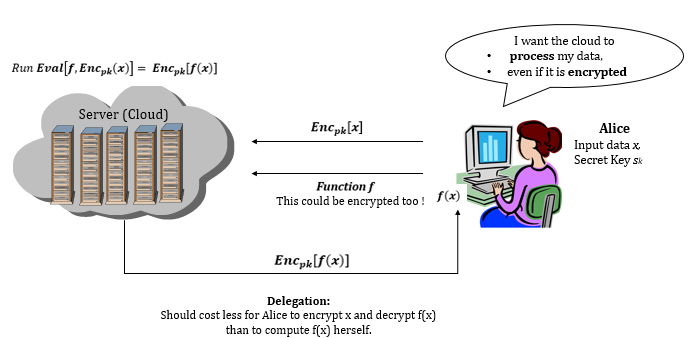
\includegraphics[width=\linewidth]{figures/fhew_prob_stmt.PNG}
 \caption{FHE: Problem Statement
 \cite{shai_he}}
 \label{fig:fhew_prob_stmt}
\end{figure}
Fully homomorphic encryption scheme $\epsilon$ involves 4 key steps:
\begin{itemize}
\item \textbf{\textit{$KeyGen_\epsilon$}($\lambda$):}
It involves generation of random odd integer \textit{p}, which is P-bits long as the secret key. The security parameter $\Lambda$ dictates the bit-length of the key.
\begin{itemize}
\item Symmetric Encryption: \\
The same secret key is used for both Encryption and Decryption.  
\item Asymmetric Encryption:\\ It is a public key encryption scheme and comprises of a public encryption key ($p_k$) and a secret decryption key ($s_k$).
\end{itemize}
\item \textbf{\textit{$Encrypt_\epsilon$}(\textit{p,m}):}\\
\underline{Required Parameters:}\\
Given the security parameter $\lambda$, \\N = $\lambda$; P = $\lambda^2$; Q = $\lambda^5$\\
\underline{Scheme:}\\
Consider a bit \textit{m} $\in$ {0,1}. \\To encrypt this bit, set \textit{m'= m mod 2}, a random N-bit number.\\
Output ciphertext: \textit{c $\leftarrow$ m' + pq}, where \textit{q} is a random Q-bit integer.\\
i.e. \textit{c $\leftarrow$ m mod 2 + pq}
\item \textbf{\textit{$Decrypt_\epsilon$}(\textit{p,c}):}\\
Output: \textit{c' mod 2}, \\where \textit{c' = c mod p} is an integer in the range \textit{(-p/2, p/2)} and \textit{p} divides \textit{c-c'}.\\
\textit{c - c' = c - c mod p = c (1 - mod p)} is divisible by \textit{p}. Hence, the ciphertexts of $\epsilon$ are near-multiples of \textit{p} as is observed in \cite{gentry2010computing}.\\ \\Decryption necessitates a \textit{compact ciphertext requirement}. i.e. Any two ciphertexts $c_1$ and $c_2$ outputted from the encryption scheme should be of the same size in order to maintain a constant complexity of decryption\cite{gentry2010computing}. Size of the ciphertext and the time taken to decrypt should be independent of the complexity of function \textit{f}, delegated to the cloud to compute.
\item \textbf{\textit{$Evaluate_\epsilon$}(\textit{$p_k$, f, $c_1$, $c_2$, ... $c_t$}):}\\Evaluation is associated to a set of permissible functions \textit{$F_\epsilon$}. For any function \textit{f} in \textit{$F_\epsilon$} and ciphertexts \textit{$c_1$, $c_2$... $c_t$}, where \textit{$c_i$} $\leftarrow$ \textit{$Encrypt_\epsilon$}(\textit{$p_k$, $m_i$}), the following 2 steps are performed:\\
\textit{c} $\leftarrow$ \textit{$Encrypt_\epsilon$[ f ($c_1$, $c_2$, ... $c_t$)]}\\
$Decrypt_\epsilon$(c , $s_k$) = \textit{f ($m_1$, $m_2$, ... $m_t$)}
\end{itemize}
This scheme guarantees one-wayness. i.e. given the ciphertext c, it should be very hard to output the message \textit{m} under public key $p_k$. i.e. The probability of success should be less than $\frac{1}{\lambda^k}$, for any constant \textit{k}. It also provides semantic security against chosen plain-text attacks as it is probabilistic. There can be many ciphertexts which encrypt a given message and $Encrypt_\epsilon$() chooses one at random. 
\subsubsection*{Example}
The homomorphic operations are defined as follos:\\
$Add_\epsilon$($c_1$,$c_2$) $\rightarrow$ $c_1$ +  $c_2$\\
$Sub_\epsilon$($c_1$,$c_2$) $\rightarrow$ $c_1$ -  $c_2$\\
$Mult_\epsilon$($c_1$,$c_2$) $\rightarrow$ $c_1$ .  $c_2$\\
Consider multiplication of 2 ciphertexts $c_1$ and $c_2$. $\Rightarrow$ c = $c_1$ . $c_2$\\
$c_i$'s noise is defined by $m_i$' = $m_i$ (mod 2), where $m_i$ and $m_i$' have the same parity.\\
c = $m_1$'.$m_2$' + pq' for some q'.\\
\subsubsection*{Concept of Bootstrapping}

\subsection{Existing code flow}
\label{5_1_1}

\subsection{Hot-Spots for Hardware Acceleration}
\label{5_1_2}
Profiling results have confirmed that the Homomorphic NAND operation takes up the maximum execution time. Each HomNAND operation makes several calls to Accumulator as illustrated in Table \ref{table:sw_hotspots_fhe}. The accumulator in turn calls the 2048-point FFT and IFFT routines several times.
\begin{table}[htbp]
\caption{Analysis of Software Bottlenecks}
\centering
\begin{tabular}{c p{4.5cm} c}
\toprule
HomNAND Test Count & Function & Number of function calls\\
\midrule
\multirow{4}{*}{0}&FFT&396002\\
\cmidrule(r{4pt}){2-3}
  &Inverse FFT&132000\\
\cmidrule(r{4pt}){2-3}
 &Homomorphic NAND&0\\
\cmidrule(r{4pt}){2-3}
 &Add to Accumulator&0\\
\midrule
\multirow{4}{*}{1}&FFT&499430\\
\cmidrule(r{4pt}){2-3}
 &Inverse FFT&166470\\
\cmidrule(r{4pt}){2-3}
 &Homomorphic NAND&3\\
\cmidrule(r{4pt}){2-3}
 &Add to Accumulator&2872\\
\bottomrule
\end{tabular}
\label{table:sw_hotspots_fhe}
\end{table}
The tabulated values are averages obtained from 5 runs of the application in each of the two cases, HomNAND Test for 0 and 1 rounds. The number of function calls is not deterministic but usually around a certain range, due to the random nature of input, secret and bootstrapping keys. Each HomNAND Test involves 3 HomNAND function calls in the implemented FHE design \cite{fhew_lib} \ref{table:sw_hotspots_fhe}. This is because the circuit under test is defined by: (\textbf{a} NAND \textbf{b}) NAND (\textbf{c} NAND \textbf{d}).\newline \newline
The table[] illustrates the average execution time of a single FFT and IFFT, taken across --readings in a quad-core CPU. Since maximum calls are made to FFT and IFFT functions, porting these portions to hardware might facilitate parallel execution as opposed to sequential flow in software and speed it up further. Embedded devices are usually memory and power constrained. In the latest patch of FHEW Library \cite{fhew_lib}, the FFTs are computed on double-precision floating point values which are 64 bits long. Hence, exploring the accuracy of results with varying bit-widths is another interesting aspect to investigate, for a holistic analysis of hardware acceleration using FPGAs. These experiments shall also be covered in the forthcoming sections of this thesis.
\subsection{Hardware Results}
\label{5_1_2}

\subsection{Comparative Analysis of results from software and hardware}
\label{5_1_3}